\section{A rational counterexample}
In this section we prove that a statement as in theorem \ref{thm:Hbms*as*ggrep}
cannot hold if we consider homology with coefficients in $\Q$. We still don't know
if the analogue of theorem \ref{thm:main} holds in homology with coefficients in $\Q$
or in fields of odd characteristic.

We recall that $H_*(C_m(\Sigma_{g,1});\Q)$ has been computed \emph{as a bigraded $\Q-$vector space}
by B\"odigheimer, Cohen and Milgram in \cite{BCM}, and more recently by Knudson in \cite{Knudson}. A description of
these homology groups as a
$\gg-$representation seems to be still missing in the literature.

We will prove the following theorem:
\begin{thm}
 \label{thm:counterexample}
 Let $g\geq 2$ and $m\geq 2$; then $H_2(C_2(\Sigma_{g,1});\Q)$ is not a symplectic
 representation of $\gg$.
\end{thm}
\begin{proof}
 Let again $\S=\Sigma_{g,1}$. We will use the following strategy:
 \begin{itemize}
  \item we define a homology class $[a]\in H_2(C_2(\S);\Q)$ represented by a cycle $a$;
  \item we prove that $[a]\neq 0$ by computing the algebraic intersection of
  $[a]$ with a homology class
  in $\tH_2(\cms^c;\Q)$; here it is worth stressing that the manifold
  $\cms$ is orientable: therefore we can apply Poincaré-Lefschetz duality
  also with rational coefficients;
  \item we define another homology class $[b]\in H_2(\cms;\Q)$ and show that
  $[b]$ is mapped to $[b]+2[a]$ by some element in the Torelli group $\mathcal{I}_{g,1}$.
 \end{itemize}
Recall that the Torelli group $\mathcal{I}_{g,1}$ is the kernel of the surjective homomorphism
$\gg\to Sp_{2g}(\Z)$; if an element of the Torelli group acts non-trivially on
some class in $H_2(C_2(\S);\Q)$, then this is not a symplectic representation of $\gg$.

We consider again $\T(\S)$ as model for $\mrS$. Let $c$ be an simple closed curve
representing the homology class $\u_1$, and assume that $c$ intersects $\U_1$ once
transversely and is disjoint from all other $\U_i$'s and from all $\V_i$'s. Let $c'$
be a parallel copy of $c$.

We consider the torus $a=c\times c'$ of configurations in $C_2(\S)$ having one point lying on $c$ and
one lying on $c'$: by abuse of notation, denote also one of its fundamental cycles by $a$
(there are two possible choices, corresponding to the two possible orientations of $a$).

Let $\tup=(0,(u_i,v_i))$ with $u_1=2$ and all other $u_i$'s, as well as all $v_i$'s, equal to zero.
Then the map
\[
\phi_{\tup}\colon (\Delta^{\tup},\partial\Delta^{\tup})\to (C_2(\S)^c,\infty)
\]
maps the fundamental class in $H_2(\Delta^{\tup},\partial\Delta^{\tup};\Q)$ to a homology
class in $\tH_2(C_2(\S)^c;\Q)$.
% ; if we see $e^{\tup}$ as a properly embedded, orientable submanifold
% of $C_2(\S)$, then we are just considering its fundamental class $[e^{\tup}]\in H_2(C_2(\S)^c)$.

The cell $e^{\tup}$ intersects once, transversely the torus $a$, therefore the
algebraic intersection $[a]\cap[e^{\tup}]$ is $\pm 1$,
where the signs depends on how we have chosen orientations on $a$, $e^{\tup}$ and $C_2(\S)$ itself;
in particular $[a]\neq 0$.

The action of $\gg$ on isotopy classes of simple closed curves is transitive, so we can repeat
the construction of the torus $a$ with any other copy of parallel, non-separating simple closed curves
$c$ and $c'$, and the resulting class $[a]$ will always be non-trivial in $H_2(C_2(\S);\Q)$.

See figure \ref{fig:rational} to visualize the following discussion.
Let $d$ and $d'$ be disjoint, non-separating simple closed curves such that
cutting $\S$ along $d$ and $d'$ we obtain a subsurface $\S'\simeq\Sigma_{1,2}$ of genus 1, with boundary
components $d$ and $d'$ (here we need that the genus of $\S$ is at least 2);
suppose moreover that $c$ is a non-separating simple closed curve in $\S'$,
and let $c',c''$ be two parallel copies of $c$ in $\Sigma_{1,2}$, one on each side of a small tubular
neighborhood of $c$.
Then $d,d',c',c''$ are the boundary of a subsurface $\S''\simeq\Sigma_{0,4}\subset\S'$.
Orient all curves $d,d',c,c',c''$ in such a way that the following equalities hold:
\begin{itemize}
 \item $[d]=[d']\in H_1(\S;\Q)$, as witnessed by the subsurface $\S'$;
 \item $[c]=[c']=[c'']\in H_1(\S;\Q)$;
 \item $[d]-[d']+[c']-[c'']=0\in H_1(\S\setminus c;\Q)$, as witnessed by the subsurface $\S''$.
\end{itemize}

\begin{figure}\centering
 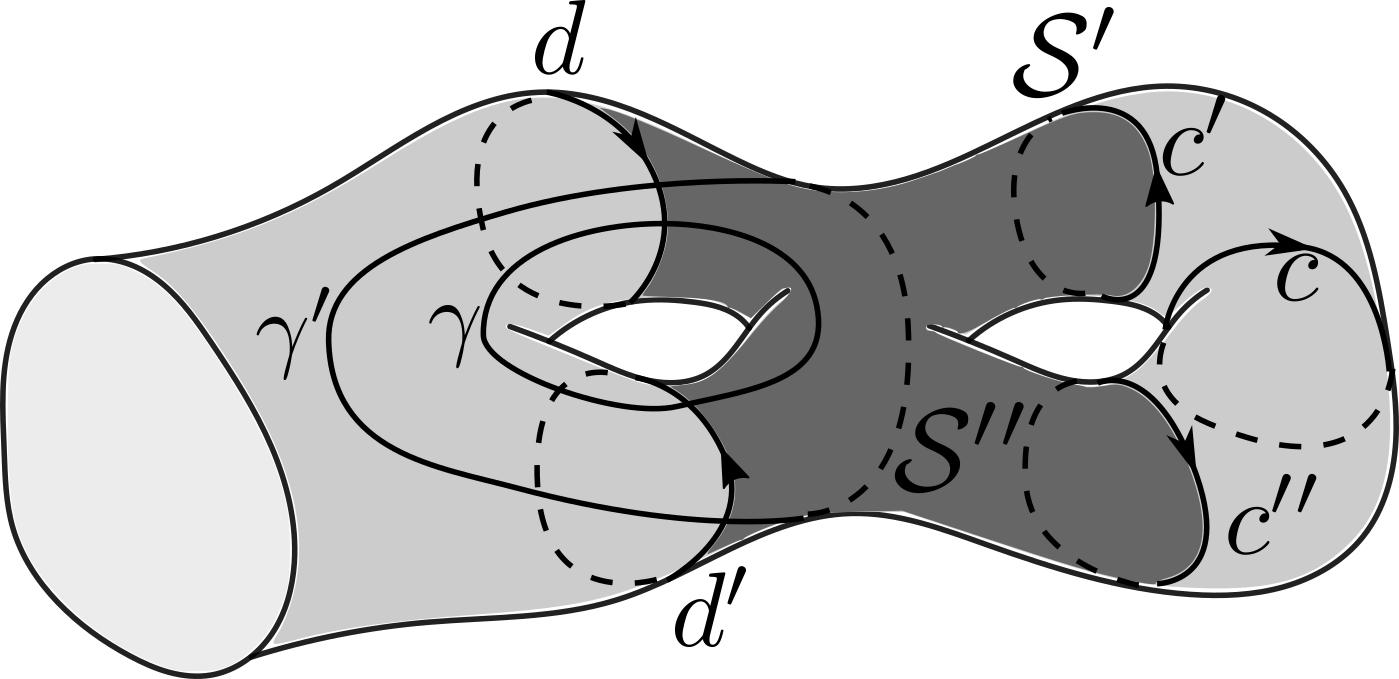
\includegraphics[scale=1.0]{figures/rational.png}
 \caption{The curves $d,d',c,c',c'',\gamma,\gamma''$ and the subsurfaces $\S',\S''$.}
\label{fig:rational}
\end{figure}

The four tori $c\times c'$, $c\times c''$, $c\times d$ and $c\times d'$ are contained in $C_2(\S)$
and the equality
\[
 [c\times d]-[c\times d']+[c\times c']-[c\times c'']=0\in H_2(C_2(\S))
\]
holds, as witnessed by the homology $c\times \S''\subset C_2(\S)$.

Moreover the classes $[c\times c']$ and $-[c\times c'']$ are \emph{equal}:
indeed there is an isotopy of $\S$ mapping $c$ to $c'$ and $c''$ to $c$,
as oriented curves; the class $[c\times c'']$ is mapped to the class $[c'\times c]=-[c\times c']$.

Let again $a=[c\times c']$ and let $b=[c\times d]$: then the class $b'=[c\times d']$
is equal to $b+2a\in H_2(C_2(\S);\Q)$.

Consider now an element of the Torelli group that fixes $c$ and maps $d$ to $d'$ preserving
the orientation, for example the bounding pair $D_{\gamma}\circ D_{\gamma'}^{-1}$, where
$\gamma$ and $\gamma'$ are represented in figure \ref{fig:rational}:
then the class $b$ is mapped to $b'=b+2a\neq b$.
\end{proof}

The previous proof works word by word if we replace $\Q$ by any field of odd characteristic. Moreover
all the arguments in the previous proof can be adapted to show that $H_*(F_2(\S);\mathbb{F})$ is
not a symplectic representation of $\gg$, where $F_2(\S)$ is the ordered configuration space
and $\mathbb{F}$ is \emph{any} field, including $\Z_2$. The result of theorem \ref{thm:Hbms*as*ggrep}
is peculiar of unordered configurations and characteristic 2.